Navrhněte pravidla pro oboustranný převod mezi oběma formami ve spisovné češtině.


\section{First-person to Third-person Rules}
In First-person $\rightarrow$ Third-person conversion direction, I have proposed four rules. These four rules cover:
	\begin{itemize}
		\item Personal pronouns replacement
		\item Possesive pronouns replacement
		\item Replacement of contidional, present and future verb forms, conjunctions
		\item Auxiliary verbs replacement or deletion
	\end{itemize}

In this section, I describe each of these rules.

\subsection{Personal pronouns}

This rule covers the conversion of a personal pronoun \emph{já (I)} and its forms. The pronoun can be replaced by:
	\begin{itemize}
		\item another pronoun -- \emph{ona (she)}/\emph{on (he)}
		\item noun -- usually a proper noun, given as the protagonist's name
	\end{itemize}

In both cases, the replacement must be in a corresponding form to keep a sentence grammatically correct.

The rule is illustrated in a diagram \ref{fig:icher-perspron-rule}.

\begin{figure}[!htbp]
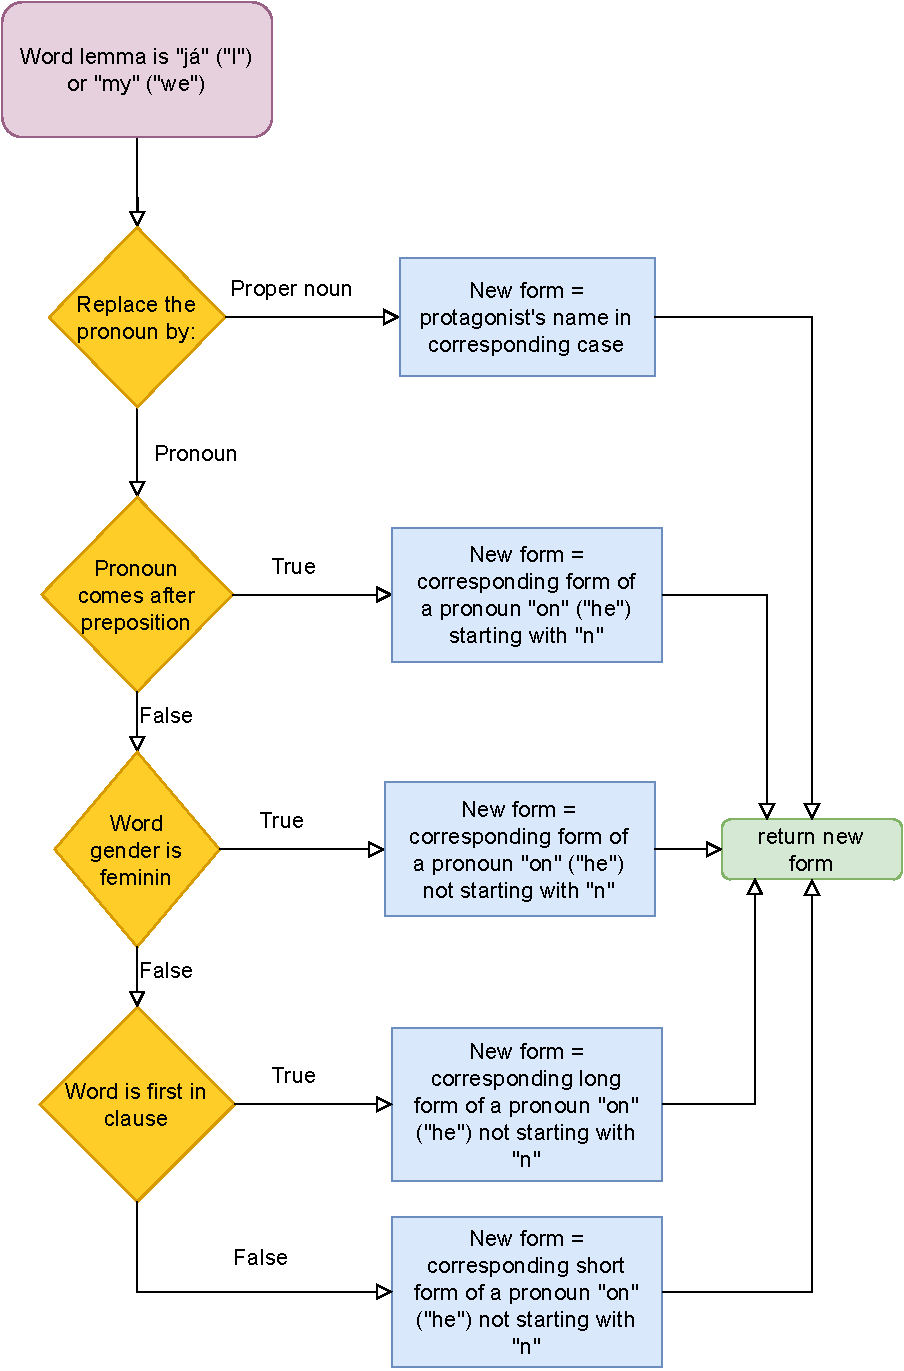
\includegraphics[width=\textwidth]{data/Icher-Perspron-Rule.pdf}
\caption{Personal pronouns replacement rule}
\label{fig:icher-perspron-rule}
\end{figure}

\subsection{Possessive pronouns}

In addition to personal pronouns, possessive pronouns must also be converted. The process is similar to the previous one. The goal is to convert a possessive pronoun \emph{můj (my)} and its forms to possessive pronouns \emph{její (her)} / \emph{jeho (his)}, or the possessive form of a proper noun. Considering the limits given by the morphological analyzer, I have decided not to include the second type of replacement. Therefore all the possessive pronouns would be replaced by possessive pronouns.

The rule is illustrated in a diagram \ref{fig:icher-posspron-rule}.

\begin{figure}[!htbp]
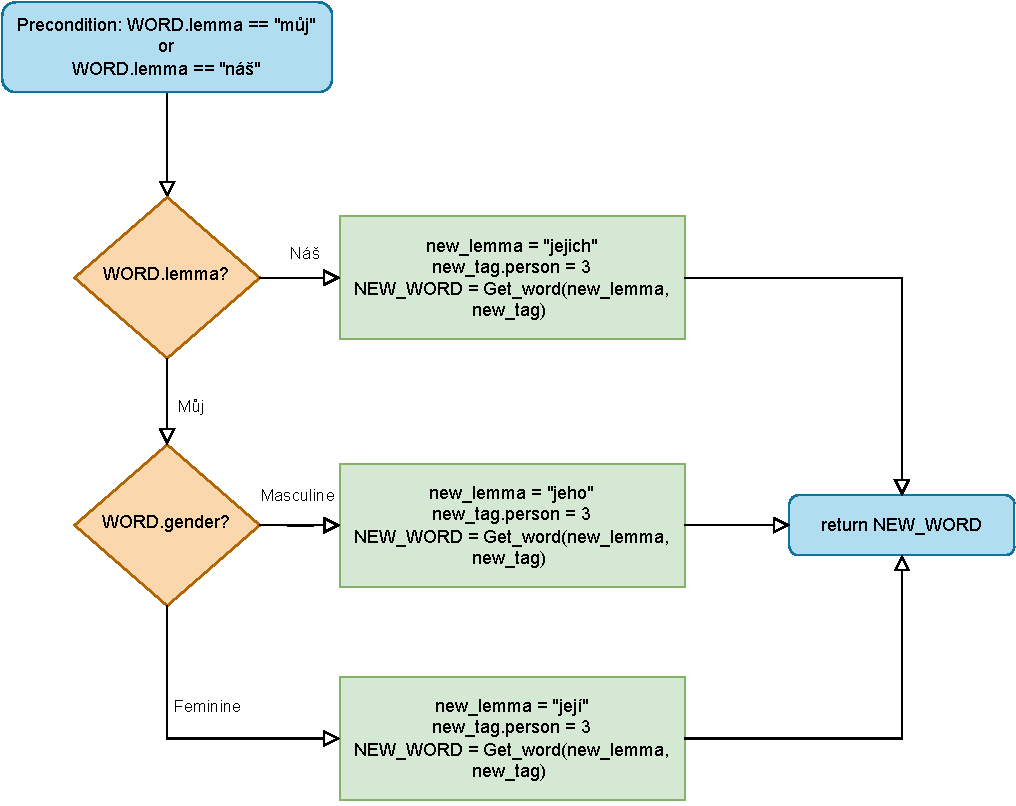
\includegraphics[width=\textwidth]{data/Icher-Posspron-Rule.pdf}
\caption{Possessive pronouns replacement rule}
\label{fig:icher-posspron-rule}
\end{figure}

\subsection{Conditionals, indicatives, conjunctions}

The third rule covers several cases. This is because the conversion procedure is same in all cases. The process is simple: we just need to change the person in the word's tag, and then generate a new word form from this new tag and the original lemma, as shown in \ref{fig:icher-predicate-rule}.

To put it simply, this rule includes these types of conversion:
\begin{itemize}
	\item bych/bychom $\rightarrow$ by -- \emph{conditional auxiliary verbs}
	\item budu/budeme $\rightarrow$ bude/budou -- \emph{future indicatives}
	\item píšu/píšeme $\rightarrow$ píše/píšeme -- \emph{example of present indicative}
	\item abych/abychom/kdybych/kdybychom $\rightarrow$ aby/kdyby -- \emph{conjunctions}
\end{itemize}


\begin{figure}[!htbp]
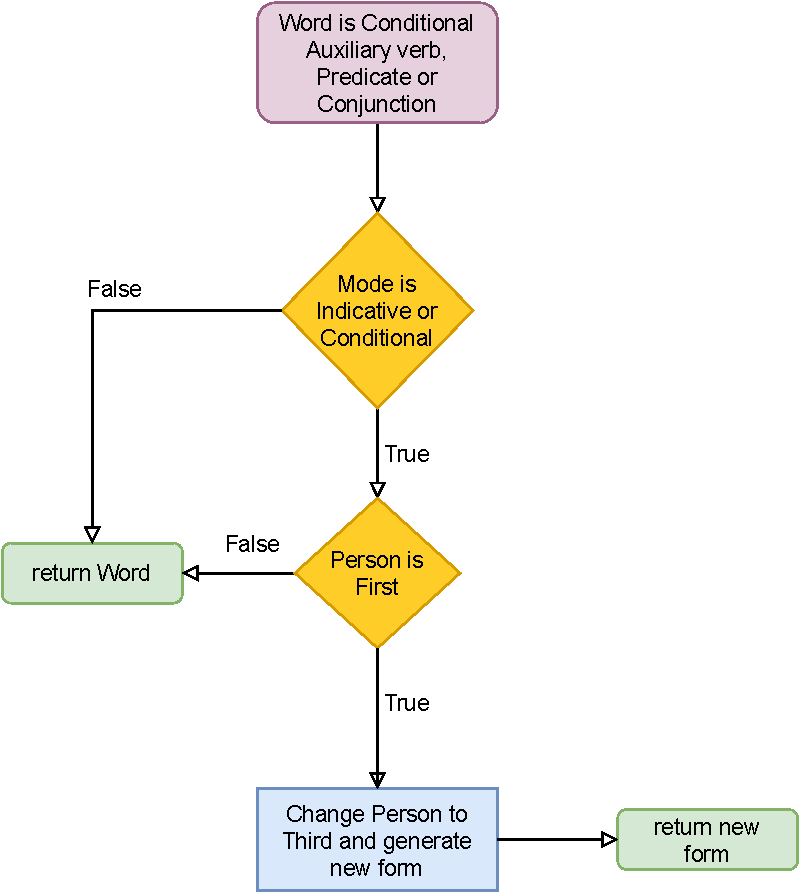
\includegraphics[width=\textwidth]{data/Icher-Predicate-Rule.pdf}
\caption{Rule replacing the conditionals, conjunctions and verb forms in present indicative tense and future indicative tense}
\label{fig:icher-predicate-rule}
\end{figure}

\subsection{Auxiliary verbs}

Finally, we need to replace or delete other auxiliary verb. If the participle that auxiliary verb depends on, the auxiliar should be deleted. However, if the participle is passive, the auxiliar should be kept and converted.

For example, a sentence \emph{Ukradl \textbf{jsem} klávesnici (I stole a keyboard)} converts to \emph{Ukradl klávesnici (He stole a keyboard)}, but \emph{\textbf{Jsem} ukradena (I am stolen)} should convert to \emph{\textbf{Je} ukradena (She is stolen)}.

Also, the auxiliary verb needs to be in indicative mode to be converted. The conditional verbs are covered in the previous rule. Then, there are other modes of auxiliary verbs that should not be converted at all, as the auxiliar in plusquamperfect. For instance, a sentence \emph{\textbf{Byl jsem} ukradl klávesnici} might convert to \emph{Juraj \textbf{byl} ukradl klávesnici}. As we can see, the sentence in the first-person narrative contains two auxiliary verbs, however, only the one in indicative mode would be deleted.

I present the rule in \ref{fig:icher-auxverb-rule}.

\begin{figure}[!htbp]
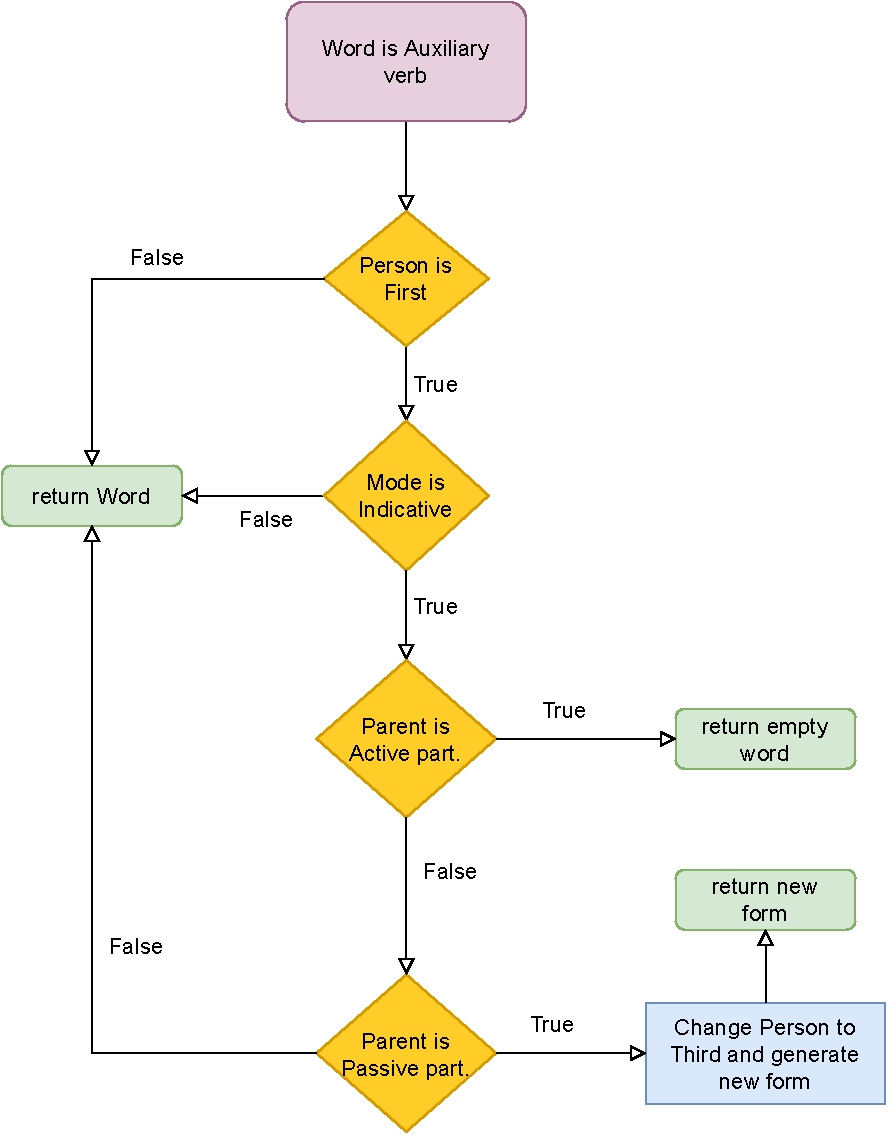
\includegraphics[width=\textwidth]{data/Icher-Auxverb-Rule.pdf}
\caption{Rule replacing the indicative forms of auxiliary verbs}
\label{fig:icher-auxverb-rule}
\end{figure}

\section{Third-person to First-person Rules}

Since this direction is much more complicated for conversion than the other one, I propose seven rules which cover:

\begin{itemize}
	\item Proper nouns replacement
	\item Predicates replacement
	\item Conditional auxiliars replacement
	\item Auxiliary verbs addition or replacement
	\item Personal pronouns replacement
	\item Possessive pronouns replacement
	\item Conjunction replacement
\end{itemize}

\subsection{Proper nouns}

\subsection{Predicates}

\subsection{Conditional auxiliars}

\subsection{Indicative auxiliars}

\subsection{Personal pronouns}

\subsection{Possessive pronouns}

\subsection{Conjunctions}
